\section*{The Speech engine}
\subsection*{Which Speech Engine did we use ?}
There exist a lot of speech recognition engines available on the market \cite{list_rec_soft}. Among all the possible one, we especially studied the qualities and defaults of three different speech engines to choose the one to use on our application. 

First we looked at ATK the real-time API for HTK \cite{atk}. This API was build to facilitate building experimental application for HTK. It consists of a C++ layer lying on the top of the standard HTK library. ATK was, like HTK, developed at the departement of engineering in the university of Cambridge. A good point of using ATK is that it enables us to easily build and train a recognizer from scratch. However, ATK had some defaults which prevented us to use HTK as a speech engine for the game. First of all the last update of ATK date back to 2007 and not much available documentation on the web which let us fear some troubles. Moreover, ATK does not support Mac. 

It was also conceivable to use Google's Web Speech API \cite{google_speech_api}. One of the main strength of Google's Web Speech API is that it is very accurate and quick. However, Google Web Speech API is not open source and only access to a demonstration version of it is possible for free. Moreover, using the Web Speech API would have forced  the user to have access to internet while playing the game which is not very practical. 

The solution we finally chose was to use CMUSohinx. Sphinx is a group of open-source speech recognition systems developed at Carnegie Mellon University \cite{sphinx}. In particular, among Sphinx package, used Sphinx4. Sphinx4 is an adjustable, modifiable recognizer written in Java. Since Sphinx4 is entirely developed in Java it makes it easy to link the recognizer to the rest of the game. The main quality of Sphinx4 is that it is is quite easy to use, with anough available tutorial and explanation and very flexible. Sphinx4 enables us to define our own dictionary and our own grammar for example. 

\subsection*{How does Sphinx4 work ?}
Sphinx speech recognition system has three elements : the Front End , the Knowledge base and the decoder . Front End receives and processes speech signals. Knowledge base provides data for decoder and the decoder performs the recognition itself. Figure \ref{fig:sphinx_struc} presents in a visual way the structure of Sphinx recognizer. 

In the following, we now look more closely each component of Sphinx. 

\begin{figure}[h!]
\center{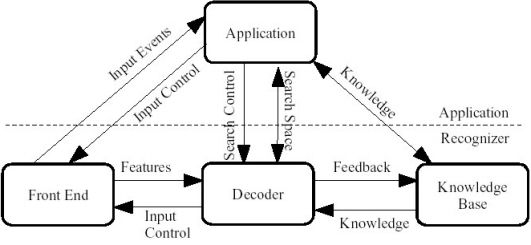
\includegraphics[width=0.8\linewidth]{sphinx_structure.png}}
\caption{Sphinx Structure. \cite{understand_sphinx}}
\label{fig:sphinx_struc}
\end{figure}

\subsubsection*{The Front End : Spectral analysis and feature extraction}
The Front End is responsible for processing the input signal so as to give the decoder understandable information. The waveform of the signal is split into utterances. Utterances are separated by silences. Then, sphinx uses basically frame-base processing, i.e one utterance is regularly divided into frame of length 10ms before features are extracted from each frame. The feature vector is typically of length 39. The vector features used in Sphinx are extracted from spectral analysis of the frame. There are : the Mel Frequency Cepstrum Coefficients, there derivative and second derivative in time (Delta coefficient and Delta-delta) and the power coefficient (or energy) with its derivative. Figure \ref{fig:sig_proc_sphx} resumes this processing. 

\begin{figure}[h!]
\center{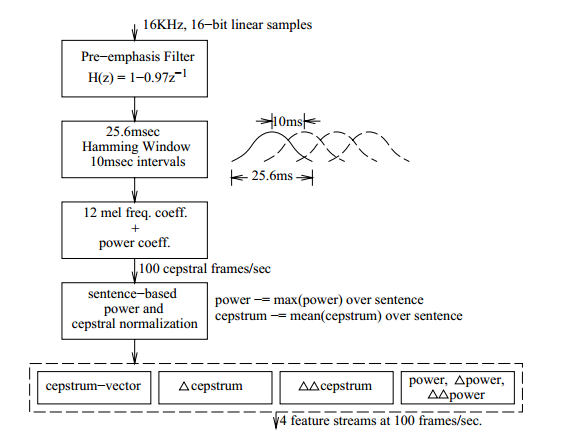
\includegraphics[width=0.8\linewidth]{signal_proc_sphinx.png}}
\caption{Signal processing in the Front End of Sphinx. \cite{eff_algo}}
\label{fig:sig_proc_sphx}
\end{figure}

\subsubsection*{The knowledge base : Different models}
The knowledge base contains three different models which will then be used by the decoder to match the given list of feature vector to the most probable sentence. Different models are used depending on the application (language, possible vocabulary...).  

\textbf{The acoustic model}

The goal of the acoustic model is to represent the probability of a sound given a segment. In Sphinx, each phoneme is formed with five segments or state. Depending on the wideness of the vocabulary, the memory and the accuracy requirement in our application we may use either context-independent or context-dependent models. Context-dependent models aims to represent co-articulation  by duplicating each phoneme model depending on its left and right context : triphone. Acoustic models are heavily dependent on the language and on the the way of recording. With Sphinx full acoustic models have already been trained in several languages and different recording context. It is however possible to train its own acoustic model using SphinxTrain. 

Context-independent phones and triphones in the acoustic model are represented via continuous density hidden Markov models (Figure \ref{fig:HMM}) where the transitions probabilities in the model are approximated by Gaussian mixtures. In fact, Sphinx uses semi-continuous modelling with clustering. For fully continuous HMMs, each state in the HMM (i.e each phone or tri-phone) need its own separate weighted Gaussian mixture which is computationally and memory expensive. In Sphinx, the states are are grouped into cluster called senones. Each senone is represented by a single Gaussian misture codebook but inside the senone each state is represented by its own mixture weights. 

All the parameters of the HMMs are evaluated through a modified version of the Baum-Welch algorithm. 


\begin{figure}[h!]
\center{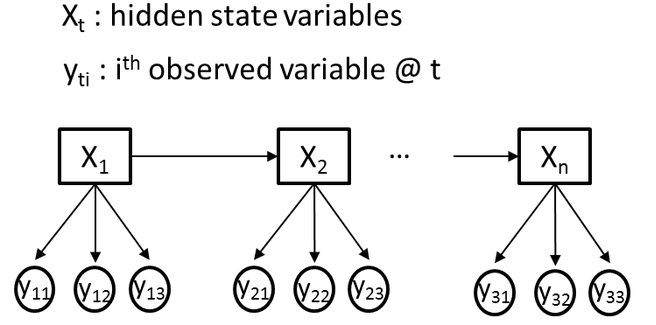
\includegraphics[width=0.5\linewidth]{HMM.png}}
\caption{Hidden Markov Model}
\label{fig:HMM}
\end{figure}

\textbf{The lexical model}

The lexical model in sphinx consist in a phonetic dictionary. It contains a mapping from word to phones. This mapping is not very efficient because only two to three pronunciation variants are noted in it, but it's practical enough most of the time. The dictionary is not the only variant of mapper from words to phones. It could be done with some complex function learned with a machine learning algorithm. 

\textbf{The language model}
 
The language model or grammar enables the recognizer to choose the most likely word sequence given the sounds and the previously recognized words. The language model is key in the recognition process because it make it possible to significantly restrict the search space. By default, Sphinx uses tri-grams, i.e one compute the probability of one word occurrence given the two previous ones and forget about earlier words.  

\subsubsection*{The decoder : Recognition itself}
The decoder performs the main part of the speech recognition. It reads features from the front 
end, couples this with data from the knowledge base, and performs a search to determine the most likely sequences of words that could be represented by the series of features output by the Front End.

Sphinx recognition system has a three-pass decoder structure. The first pass consist in a forward Viterbi beam search perform on the full vocabulary. The result of this search is a single recognition hypothesis and word lattice that contains all the words recognized during the search. The second pass is a time synchronous Viterbi beam search in the backward direction. This search is restricted to the word identified in the first pass and is thus very fast. The last pass is an A* or stack search using the word segmentations and scores produced by the
forward and backward Viterbi passes above. This pass output a list of the most likely hypothesis.